\documentclass[letterpaper,12pt]{report}
\usepackage{pstricks}
\usepackage{amsmath}
\usepackage{wrapfig}
\usepackage{graphicx}

\begin{document}


% Title
\title{ Force Control of an RPR manipulator\\EL 522 Final Project}
\author{Griswald Brooks}
\maketitle
 
\begin{abstract}
While positioning of manipulator end effectors is an important task, often applying a particular force to the environment is needed.
This paper describes a basic hybrid force control technique and presents simulation results.
\end{abstract}

\tableofcontents

\chapter{Introduction}

\section{Concept and Motivation} \label{sec:concept}
Many manipulator applications require specific amounts of force to be applied to the environment. 
Tasks include machining, object manipulation, and part assembly. 
Without force control, the robot would apply an arbitrary amount of force as a function 
of its joint error and interaction with the environment. This would lead to unpredictable
results and possible manipulator instability, e.g. causing the end effector to bounce or damage
the object or environment with which it's interacting.

One method of force control is a feed forward method called impedance control. In this method 
the environment is modeled as a mass-spring or a mass-spring-dampened system 
and the required displacement needed for a desired force is calculated \eqref{eq:displacementeq1}. 
The manipulator is then commanded to its intended tracking plus this displacement. This can be thought of
as the manipulator tracking an inner virtual wall.


\begin{equation} \label{eq:displacementeq1}
\delta x = \frac{F_d}{k}
\end{equation}

\begin{figure}
\centering
% Spring
\def\zigzag{\psline(0,0)(0.5,0.5)(1.5,-0.5)(2,0)}
\psset{unit=0.25,linewidth=1.5pt}
\multips(-1,0)(2,0){4}{\zigzag}
\psline[linewidth=1.5pt](-2,0)(-1,0)
\psline[linewidth=1.5pt](8,0)(7,0)
% Spring label
\rput(4.5,2.5){$k$}
% Virtual Wall
\psline[linewidth=1.5pt,linestyle=dashed, dash=3pt 3pt](1,-3)(1,3)
% Ground
\pspolygon[linecolor=white,fillstyle=hlines](8,-3)(8,3)(8.9,3)(8.9,-3)
\psline[linewidth=1.5pt](8,-3)(8,3)
% Wall
\psline[linewidth=1.5pt](-2,3)(-2,-3)
% Force arrow
\psline[linewidth=3pt]{->}(-5,2)(1,2)
% Force label
\rput(-7,2){$F_d$}
% dx arrow
\psline[linewidth=1pt]{<->}(-2,-1.75)(1,-1.75)

% dx label
\rput(-.5,-1){$\delta x$}

\caption{Mass-spring wall model with virtual wall.}
\end{figure}


Where $F_d$ is the desired force, $k$ is the modeled wall spring constant, and $\delta x$ is the wall displacement necessary to produce $F_d$.
One drawback of this method is that it assumes perfect knowledge of the environment. If the wall stiffness varies the applied force will vary.
To supplement this, a force/torque sensor can be added to the end effector which provides feedback to the controller allowing the applied force
to be modulated. This method is known as Hybrid Force Control and is the technique used in this report.

\section{Manipulator Model}

The manipulator considered in this project is the RPR manipulator. It has a revolute joint at its base and wrist which are coplanar, 
and a prismatic joint in between, Figure \ref{fig:RPRfig}. 

\begin{figure}[t]
\centering
% link 1&2
\pspolygon[linewidth=1.5pt](-2.0884,0.3384)(-1.9116,0.1616)(0.2097,2.2829)(0.0329,2.4597)
% link 3
\pspolygon[linewidth=1.5pt](0.1213,2.4963)(0.1213,2.2463)(3,2.2463)(3,2.4963)
% base block
\pspolygon[linewidth=1.5pt](-1.75,-0.25)(-2.25,-0.25)(-2.25,0.25)(-1.75,0.25)
% joint 2
\pspolygon[linewidth=1.5pt,fillstyle=solid](-0.5858,2.0178)(-0.2322,1.6642)(-1.8232,0.0732)(-2.1768,0.4268)
\pspolygon[linewidth=1.5pt,fillstyle=solid](-0.8156,1.6112)(-0.6388,1.4344)(-1.0631,1.0101)(-1.2399,1.1869)
\pspolygon[linewidth=1.5pt,fillstyle=solid,fillcolor=black](-1.2399,1.1869)(-1.0631,1.0101)(-1.2752,0.7980)(-1.4520,0.9748)
% joint 1
\pscircle[linewidth=1.5pt,fillstyle=solid](-2,0.25){0.25}
\pscircle[linewidth=1.5pt,fillstyle=solid,fillcolor=black](-2,0.25){0.1}
% joint 3
\pscircle[linewidth=1.5pt,fillstyle=solid](0.1213,2.3713){0.25}
\pscircle[linewidth=1.5pt,fillstyle=solid,fillcolor=black](0.1213,2.3713){0.1}
% manipulator
\pspolygon[linewidth=1.5pt](3,2.7463)(3,1.9963)(3.5,1.9963)(3.5,2.2463)(3.25,2.2463)(3.25,2.4963)(3.5,2.4963)(3.5,2.7463)
\caption{Schematic diagram of RPR manipulator}
\label{fig:RPRfig}
\end{figure}

\subsection{Kinematics} \label{sec:Kinematics}
The kinematic model of the manipulator is given by the transformation matrices
\eqref{eq:Amatrices}, resulting in an end effector transformation of \eqref{eq:A1A2A3}. The DH parameters for the 
manipulator are given in Table \ref{tab:DHtable}.

\begin{subequations}
		\begin{equation}
		A_1 = 
		\begin{bmatrix}
			cos\theta_1&0&sin\theta_1&0\\
			sin\theta_1&0&-cos\theta_1&0\\
			0&1&0&0\\
			0&0&0&1\\
		\end{bmatrix}
		\end{equation}
		\begin{equation}
		A_2 = 
		\begin{bmatrix}
			1&0&0&0\\
			0&0&1&0\\
			0&-1&0&d_2\\
			0&0&0&1\\
		\end{bmatrix}
		\end{equation}
		\begin{equation}
		A_3 = 
		\begin{bmatrix}
			cos\theta_3&-sin\theta_3&0&a_3cos\theta_3\\
			sin\theta_3&cos\theta_3&0&a_3sin\theta_3\\
			0&0&1&0\\
			0&0&0&1
		\end{bmatrix}
		\end{equation}
\label{eq:Amatrices}
\end{subequations}
\begin{equation}
A_1A_2A_3 = 
		\begin{bmatrix}
			c_{13}&-s_{13}&0&a_3c_{13}+d_2s_1\\
			s_{13}&c_{13}&0&a_3s_{13}-d_2c_1\\
			0&0&1&0\\
			0&0&0&1
		\end{bmatrix}
\label{eq:A1A2A3}
\end{equation}
\begin{table}
\centering
	\begin{tabular}{r|c c c c}
		Joint&$\alpha_i$&$a_i$&$d_i$&$\theta_i$\\
		\hline
		1&0&$90^\circ$&0&$\theta_1$\\
		2&0&$-90^\circ$&$d_2$&0\\
		3&$a_3$&0&0&$\theta_3$
	\end{tabular}
\caption{DH parameters for RPR manipulator.}
\label{tab:DHtable}
\end{table}

Using the standard input tranformation matrix seen in \eqref{eq:Hin},the inverse kinematics
of the manipulator are given by \eqref{eq:IK}. These were used to calculate the desired joint positions,
given an end effector reference trajectory.
\begin{equation}
H_{in} = 
	\begin{bmatrix}
		r_{11}&r_{12}&r_{13}&d_x\\
		r_{21}&r_{22}&r_{23}&d_y\\
		r_{31}&r_{32}&r_{33}&d_z\\
		0&0&0&1
	\end{bmatrix}
\label{eq:Hin}
\end{equation}
\begin{subequations}
	\begin{align}
		\theta_1 + \theta_3 &= atan2(r_{21},r_{11})\\
		\theta_1 &= atan2(d_x-a_3c_{13},a_3s_{13}-d_y)\\
		d_2 &= \sqrt{(d_x-a_3c_{13})^2+(d_y-a_3s_{13})^2}\\
		\theta_3 &= atan2(r_{21},r_{11}) - \theta_1
	\end{align}
\label{eq:IK}
\end{subequations}
The desired joint velocities $\dot q$ were given using the inverse Jacobian, \eqref{eq:IJ}.
This involved first calculating the Jacobian, \eqref{eq:Jacob}, and numerically calculating
the Moore-Penrose pseudoinverse.
\begin{equation}
\dot q = J^\#v
\label{eq:IJ}
\end{equation}
Where $v$ is a $6\times1$ column vector containing the three end effector translational velocities and three angular
velocities.
\begin{equation} \label{eq:Jacob}
J = 
	\begin{bmatrix}
		-a_3s_{13}+d_2c_1&s_1&-a_3s_{13}\\
		a_3c_{13}+d_2s_1&-c_1&a_3c_{13}\\
		0&0&0\\
		0&0&0\\
		0&0&0\\
		1&0&1
	\end{bmatrix}
\end{equation}

Following this, the desired joint accelerations $\ddot q$ were given by \eqref{eq:IA} and calculated
using the aforementioned inverse Jacobian and the element-wise time derivative
of the Jacobian \eqref{eq:Jdot}.
\begin{equation} \label{eq:Jdot}
\dot J = 
	\begin{bmatrix}
		-a_3c_{13}(\dot\theta_1+\dot\theta_3)+\dot d_2c_1-d_2s_1\dot\theta_1&c_1\dot\theta_1&-a_3c_{13}(\dot\theta_1+\dot\theta_3)\\
		-a_3s_{13}(\dot\theta_1+\dot\theta_3)+\dot d_2s_1+d_2c_1\dot\theta_1&s_1\dot\theta_1&-a_3s_{13}(\dot\theta_1+\dot\theta_3)\\
		0&0&0\\
		0&0&0\\
		0&0&0\\
		0&0&0
	\end{bmatrix}
\end{equation}
\begin{equation} \label{eq:IA}
\ddot q = J^\#(\dot v - \dot J \dot q)
\end{equation}

\subsection{Dynamics}
Modeling the manipulator as a collection of point masses located at the revolute joints and end effector,
the dynamics of the manipulator were given by \eqref{eq:dyn}.
\begin{equation} \label{eq:dyn}
D(q)\ddot q + C(q,\dot q) + G(q) = U + B(\dot q) + J(q)^TF
\end{equation}
Where $D(q)$ is the inertia matrix \eqref{eq:Mass}, $C(q,\dot q)$ is the centripetal vector \eqref{eq:Centrip}, $G(q)$ are all the gravity terms 
\eqref{eq:Grav}, $U$ is the control input, $B(\dot q)$ are the dampening terms due to viscous joint friction \eqref{eq:Damp}, and $F$ is the generalized force vector of 
forces/torques applied to the end effector \eqref{eq:Force}.
\begin{equation} \label{eq:Mass}
D(q) = 
	\begin{bmatrix}
		(m_2+m_3)d_2^2+m_3a_3(1-2d_2s_3)&-m_3a_3c_3&m_3a_3(1-d_2s_3)\\
		-m_3a_3c_3&m_2+m_3&-m_3a_3c_3\\
		m_3a_3(1-d_2s_3)&-m_3a_3c_3&m_3a_3
	\end{bmatrix}
\end{equation}
\begin{equation} \label{eq:Centrip}
C(q,\dot q) = 
	\begin{bmatrix}
		2d_2\dot d_2 \dot\theta_1(m_2+m_3) + m_3a_3(\dot d_2s_3-(\dot d_2s_3+d_2c_3\dot\theta_3)(2\dot\theta_1+\dot\theta_3))\\
		m_3a_3s_3(\dot\theta_1+\dot\theta_3)^2 - (m_2+m_3)d_2\dot\theta_1^2\\
		m_3a_3(d_2\dot\theta_1\dot\theta_3c_3 - 2s_3\dot d_2\dot\theta_1)
	\end{bmatrix}
\end{equation}
\begin{equation} \label{eq:Grav}
G(q) = g
	\begin{bmatrix}
		(m_2+m_3)d_2s_1 + m_3a_3c_{13}\\
		-(m_2+m_3)c_1\\
		m_3a_3c_{13}
	\end{bmatrix}
\end{equation}
Where $m_2$ and $m_3$ are the masses at the elbow (joint 3) and the end effector respectively and $g$ is the acceleration due to gravity in $\frac m{s^2}$.
\begin{equation} \label{eq:Damp}
B(\dot q) = 
	\begin{bmatrix}
		-b_1\dot\theta_1\\
		-b_2\dot d_2\\
		-b_3\dot\theta_3
	\end{bmatrix}
\end{equation}
For this simulation, the viscous dampening coefficients were $b_1=b_2=b_3=0.1 \frac{Ns}{m}$.
\begin{equation} \label{eq:Force}
F = 
	\begin{bmatrix}
		f_x,f_y,f_z,\tau_x,\tau_y,\tau_z
	\end{bmatrix}
	^T
\end{equation}
Where $f_n$ represents a force in the $n$ direction and $\tau_n$ represents a torque along the $n$ axis. The details about the elements used
for this simulation are discussed in Section~\ref{sec:envmodel}.

\section{Environmental Model}\label{sec:envmodel}
As mentioned in Section~\ref{sec:concept}, hybrid force control is being simulated and as such, the environment with which the manipulator
is going to interact, i.e. a wall, is modeled as a mass-spring system. In addition to a reactive force in the direction normal to the wall,
a term for viscous friction $c$ is added for when the manipulator is 'dragging' against the wall. This results in a force vector applied to 
the end effector when contacting the wall of \eqref{eq:WallForce}.

\begin{equation} \label{eq:WallForce}
F_w = 
	\begin{bmatrix}
		k\delta x,-cv_y,0,0,0,0
	\end{bmatrix}
	^T
\end{equation}		
Where $\delta x$ in this case is always taken to be negative when the end effector is 'indenting' the wall.
According to specification, $k$ can take on any value from $6000 \frac Nm$ to $60,000\frac Nm$, so in simulation
the wall stiffness $k$ is taken as a random number within this range.

\begin{figure}[t]
\centering
% Spring
\def\zigzag{\psline(0,0)(0.5,0.5)(1.5,-0.5)(2,0)}
\psset{unit=0.25,linewidth=1.5pt}
\multips(2.5,0)(2,0){2}{\zigzag}
\psline[linewidth=1.5pt](1,0)(2.5,0)
\psline[linewidth=1.5pt](8,0)(6.5,0)
% Spring label
\rput(3.5,2.5){$k\delta x$}
% Wall
\psline[linewidth=1.5pt,](1,-2)(1,3)
% Ground
\pspolygon[linecolor=white,fillstyle=hlines](8,-2)(8,3)(8.9,3)(8.9,-2)
\psline[linewidth=1.5pt](8,-2)(8,3)
% Force arrow
\psline[linewidth=3pt]{<-}(1,1)(5,1)
% End effector
\pspolygon[linewidth=1.5pt](0,-0.5)(1,-0.5)(1,-1)(-0.5,-1)(-0.5,-0.5)(-0.5,2)(1,2)(1,1.5)(0,1.5)
% Link
\pspolygon[linewidth=1.5pt](-0.5,0)(-0.5,1)(-6.5,1)(-6.5,0)
% Link motion
\psline[linewidth=3pt]{<-}(-3,0.5)(-3,-2)
% Link motion label
\rput(-5,-1.5){$v_y$}
% Friction
\psline[linewidth=2.5pt]{<-}(-3,0.5)(-3,3)
% Friction label
\rput(-5,2.5){$cv_y$}
% Joint
\pscircle[linewidth=1.5pt,fillstyle=solid](-6.5,0.5){1}

\caption{Wall modeled as a mass-spring system with viscous friction.}
\end{figure}

\section{Feedback Linearization}

For position control, a Feedback Linearizing control was employed. Feedback linearization is the concept of developing
a control law that yields a linear input-output relationship within a non-linear system. In the context of the manipulator
equation this can be seen under the following control law, \eqref{eq:Ufeed}.
\begin{equation} \label{eq:Ufeed}
U = D(q)V + C(q,\dot q) + G(q)
\end{equation}
Where $q$ and $\dot q$ are the joint positions and velocities currently read by the joint encoders, and $V$ is a vector
of inputs to the control input $U$. When applied to the manipulator equation (and ignoring friction and external force 
inputs for this example) yields \eqref{eq:FeedCancel}.
\begin{subequations} \label{eq:FeedCancel}
\begin{align}
	D(q)\ddot q + C(q,\dot q) + G(q) &= U\\
	D(q)\ddot q + C(q,\dot q) + G(q) &= D(q)V + C(q,\dot q) + G(q)\\
	D(q)\ddot q &= D(q)V\\
	D(q)^{-1}D(q)\ddot q &= D(q)^{-1}D(q)V\\
	\ddot q &= V \label{eq:LinearFeed}
\end{align}
\end{subequations}
The terms $C(q,\dot q)$ and $G(q)$ are added in an attempt to cancel the torques on the manipulator due to the centripetal and gravity terms.
$D(q)$ is a positive definite matrix and hence is always invertible, allowing us to accommodate for the inertia terms. Equation \eqref{eq:LinearFeed} 
shows a linear relationship between joint accelerations $\ddot q$ and the new control input $V$. In this way we can now design a controller 
using linear feedback techniques.

A PD controller was designed for \eqref{eq:LinearFeed}. As this is a second order system, we can pick a dampening and natural frequency
to accommodate our needs. Let us pick a dampening $\zeta=1$ and a natural frequency of $\omega_n = 50 \frac{rad}{sec}$. This yields the
gain terms seen in \eqref{eq:Gains}. In order to make our equations linear in joint error, an additional $\ddot q_{ref}$ term must be added
to our control law, \eqref{eq:PDinE}, where $e = q - q_{ref}$ and $q_{ref}$ is the vector of joint positions we wish to track.
\begin{subequations} \label{eq:PDinE}
\begin{align}
	&\ddot q = K_pe + K_d\dot e + \ddot q_{ref}\\
	&\ddot e - K_d\dot e - K_p e = 0
\end{align}
\end{subequations}
\begin{subequations} \label{eq:Gains}
\begin{align}
	&K_p = -\omega_n^2 = -2500\\
	&K_d = -2\omega_n = -100
\end{align}
\end{subequations}

The final control law for position control is \eqref{eq:ControlLaw}.
\begin{equation} \label{eq:ControlLaw}
U = D(q)(K_pe + K_d\dot e + \ddot q_{ref}) + C(q,\dot q) + G(q)
\end{equation}

\section{Hybrid Force Control}

The hybrid force controller has two parts, impedance control and force feedback. The impedance controller brings the end effector
into the range of where the manipulator would have to be to apply a desired force and the feedback controller adjusts the joints as
needed in accordance with measurements from a force/torque sensor.

\subsection{Impedance Control}
As in Section~\ref{sec:envmodel}, the environment is modeled as a mass-spring system, in which case the depth needed for the end effector
to produce the desired force $f_d$, is given by $\delta x = \frac {f_d}k$. In the context of the Hybrid Force Controller, the environmental
stiffness $k$ need not be known exactly as the feedback controller will make the necessary adjustments to bring the applied force to the 
desired force. 
\subsection{Force Feedback Control}
Once the end effector is in contact with the wall, force/torque measurements of the end effector's interaction with the wall are taken. They
effect the manipulator according to \eqref{eq:dyn} through the vector $F$. In this manipulator, forces perpendicular to the wall are read
along the end effector's x-axis, and drag from moving along the wall is read as force in the y direction \eqref{eq:WallForce}. 
This manifests itself as \eqref{eq:Fvect}.
\begin{equation} \label{eq:Fvect}
F_w = [f_{w_x},f_{w_y},0,0,0,0]^T
\end{equation}
In order to construct a linear controller the transpose of the Jacobian $J^T$ will be applied to the control input of the force controller.
This will feedback linearize the force relationship to be $F_w = F_u$, where $F_u$ is the output by the force controller.
As $f_{w_x}$ will be negative when contacting the wall, force error takes the following form $e_{f_x}= f_{w_x} + f_{ref}$.
While the drag force of the wall has an effect on the manipulator it is not significant, therefore the controller will attempt
to directly compensate for it by applying the opposite force. The control law for the perpendicular force is given by \eqref{eq:ForceControlLaw}.
\begin{equation} \label{eq:ForceControlLaw}
F_{u_x} = f_{w_x} + K_{w_p}e_{f_x} + K_{w_d}\dot e_{f_x} + K_{w_i}\int e_{f_x}
\end{equation}
The $f_{w_x}$ term acts to cancel the reaction force from the wall while the PID controller then attempts to minimize the force error.
As force in this case is modeled as proportional wall displacement by the end effector, the derivative of the force error term $\dot e_{f_x}$
is proportional the the end effector velocity. This term is then implemented as $\dot e_{f_x} = v_x$ as the reference velocity is zero.

Being a second order equation, the gains can be chosen according to \eqref{eq:forceGainsDeriv}. While setting $\zeta$ to one seems like the obvious
choice, in practice this controller does not perform well. A better choice is to set $2\zeta\omega_n = \omega_n^2$. This brings the system under
the tuning of $\omega_n$ and $K_{w_d}$. The derivative term acts to dampen end effector jitter, while $\omega_n$ reduces the systems sensitivity to 
noise manifested as variability in wall stiffness.
\begin{subequations} \label{eq:forceGainsDeriv}
\begin{align}
	K_{w_d}s^2 + K_{w_p}s + K_{w_i} &= s^2 + \frac {K_{w_p}}{K_{w_d}} s + \frac {K_{w_i}}{K_{w_d}}
	&= s^2 + 2\zeta\omega_ns + \omega_n^2\\
	K_{w_p} &= 2\zeta\omega_nK_{w_d}\\
	K_{w_i} &= \omega_n^2K_{w_d}
\end{align}
\end{subequations}
A natural frequency of $\omega_n = 0.1 \frac{rad}{sec}$ and a $K_{w_d} = 50$ were chosen yielding the final gain terms in \eqref{eq:forceGains}.
\begin{subequations} \label{eq:forceGains}
\begin{align}
	K_{w_d} &= 50\\
	K_{w_p} &= K_{w_i} = \omega_n^2K_{w_d} = 0.5
\end{align}
\end{subequations}

\chapter{Results}
\begin{figure}[ht]
\centering
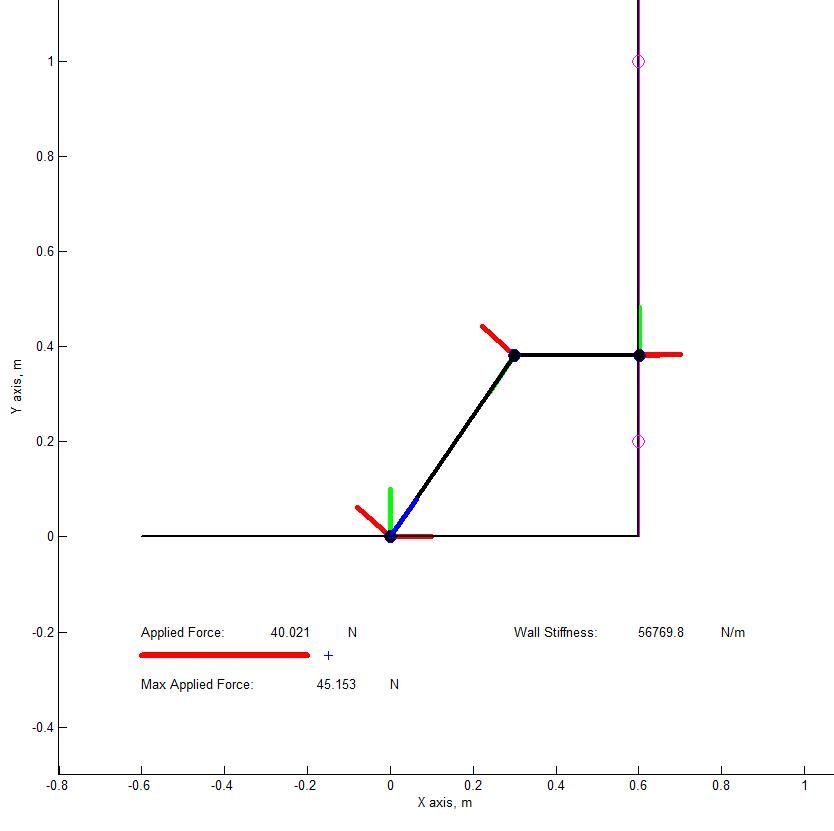
\includegraphics[width=0.6\textwidth]{SimulationImage}
\caption{MATLAB Simulation of RPR manipulator contacting wall.}
\label{fig:SimImage}
\end{figure}
The simulation was programmed to randomly choose wall stiffnesses within the allowable range (6000$\frac Nm$ to 60,000$\frac Nm$) which was then 
modulated by additive Gaussian noise in the range of 0 to 1000$\frac Nm$ for every force/torque sensor sample. The manipulator end effector was 
programmed to approach the wall in an exponential fashion in order to minimize force overshoot when colliding with the wall, and track between 
two points on the wall (0.2 m to 1 m). The manipulator used a sinusoid to track between the two points \eqref{eq:tracking}. The end effector orientation
was set to be zero, perpendicular to the wall. These trajectories were differentiated and passed to the kinematics equations, 
Section~\ref{sec:Kinematics}, producing joint position, velocity, and acceleration commands which were input to the position and force controllers.
The desired force to be applied to the wall was $F_d = 40 N$.
\begin{subequations} \label{eq:tracking}
\begin{align}
	\delta x &= \frac {F_d}{60,000} = 6.6\times10^{-4}\\
	dx &= (0.2 + \delta x)(1 - e^{-10t}) + 0.4005\\
	dy &= 0.4sint + 0.6
\end{align}
\end{subequations}
The simulation was evaluated every 0.01 seconds for 10 seconds using the RK4 method. A representative wall stiffness of $k = 56,769.7894 \frac Nm$
is used for the results of this section.

\section{Position Error}
\begin{figure}[h!b]
\centering
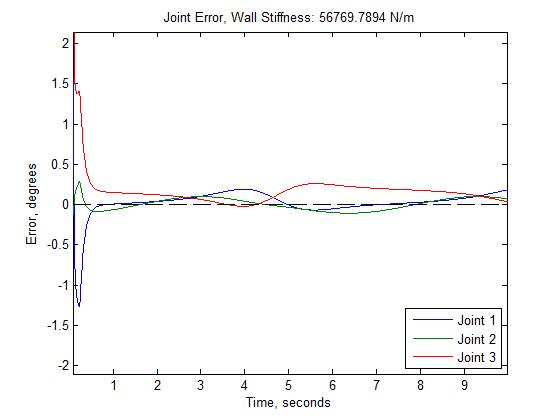
\includegraphics[width=0.6\textwidth]{JointError}
\caption{Graph of joint error over 10 seconds.}
\label{fig:JointError}
\end{figure}
The slowest joint (joint 3) reached $0.1^\circ$ joint position error in 0.5 seconds and all of the joints stayed within $\pm 0.2^\circ$ error
for the length of the simulation.

\section{Force Error}
\begin{figure}[h!b]
\centering
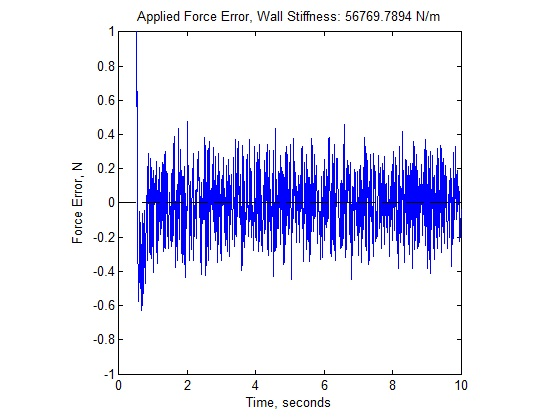
\includegraphics[width=0.6\textwidth]{AppliedForceError}
\caption{Graph of joint error over 10 seconds.}
\label{fig:ForceError}
\end{figure}
The end effector took 0.1 seconds to apply 36 N of force (90\% of $F_d$) after wall contact. The maximum force applied to the wall was 40.63 N. The force
error was $\pm 0.5 N$ proceeding the initial overshoot of 0.63 N.


\chapter{Conclusion}
Hybrid force control allows robust control over force applications in the presence of uncertain environmental conditions. It was generally tolerant of
varying environmental stiffnesses and sensor noise.
While the presented controller applies adequate force under the given specifications, a more in depth analysis of the stability of the 
force controller and the environment is necessary in order to improve its performance. 
Alternatively a Gain-Lead-Lag controller may provide increased performance over the PID controller at the expense of a small increase of controller memory.

\end{document}

The gains seemed too low for the force controller.
The inertia matrix was only positive semi-definite. 